\documentclass{ximera}

\title{Definite Integrals Activity Facilitator Guide}
\author{MATH 425: Calculus I}

\begin{document}
\begin{abstract}
   Working with the peers in your group, solve the following problems. Make sure to show and justify all your work. Make sure everyone in the group understands the solution and participates. Be prepared to report your answers to the whole class. 
\end{abstract}
\maketitle

\textbf{Student Learning Outcomes}\\
Students should be able to:
    \begin{itemize}
        \item Evaluate definite integrals geometrically from a graph or formula (that has a nice geometric interpretation).
        \item Evaluate definite integrals using the properties of definite integrals.
        \item Evaluate definite integrals using the Fundamental Theorem of Calculus.
    \end{itemize}

\textbf{Prerequisite Knowledge:} Students will need to know the interpretation of a definite integrals as the signed area between a curve and the $x$-axis.  Additionally, this activity expects students to know the properties of definite integrals and the direction of the FTC that states a definite integral is the antiderivative evaluated at the endpoints and subtracted.  If you would like to use this activity before discussing the FTC, simply omit exercise (3).\\

This activity is likely fairly short, and can be combined with the short activity on the other direction of the FTC. 

\begin{exercise}
    The given graph is a graph of the function $f(x)$. Use the graph to evaluate the definite integrals.
    %\includegraphics[scale=0.4]{Image files/5_1_5_2.png} 
    \begin{image}
        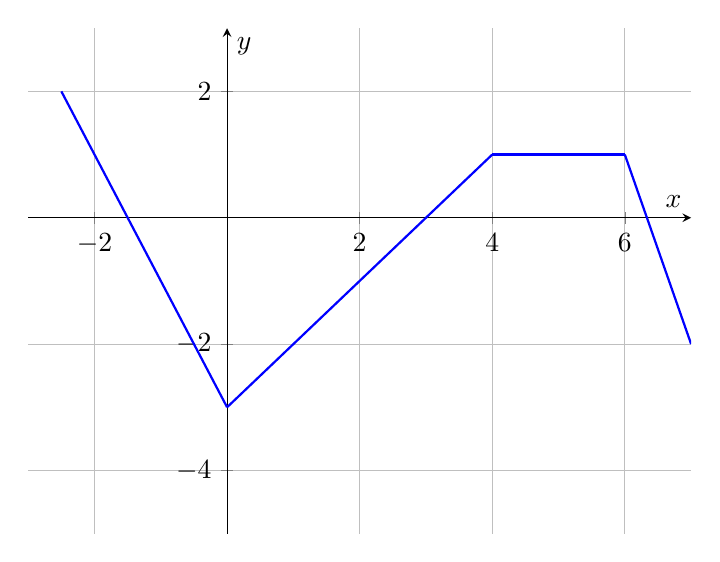
\begin{tikzpicture}
            \begin{axis}[
                axis lines = middle,
                xlabel = $x$,
                ylabel = $y$,
                xmin = -3, xmax = 7,
                ymin = -5, ymax = 3,
                grid = major,
                width = 10cm,
                height = 8cm
            ]
            
            % y = -2x - 3 for x <= 0
            \addplot[blue, thick, domain=-2.5:0] {-2*x - 3};
            
            % y = x - 3 for 0 <= x <= 4
            \addplot[blue, thick, domain=0:4] {x - 3};
            
            % y = 1 for 4 <= x <= 6
            \addplot[blue, thick, domain=4:6] {1};
            
            % y = -3x + 19 for x >= 6
            \addplot[blue, thick, domain=6:7] {-3*x + 19};
            
            \end{axis}
        \end{tikzpicture}
    \end{image}
       \begin{enumerate}
        \item $\displaystyle \int_{-2}^{0} f(x)dx$ \textcolor{blue}{$=\frac{1}{4}-\frac{9}{4}=-2$}
        \item $ \displaystyle\int_{0}^3 f(x) dx$ \textcolor{blue}{ $=-\frac{9}{2}$}
        \item $\displaystyle\int_0^4f(x) dx$ \textcolor{blue}{ $=-\frac{9}{2}+\frac{1}{2}=-2$}
        \item $\displaystyle\int_0^6 f(x) dx$ \textcolor{blue}{ $=-\frac{9}{2}+\frac{1}{2}+2=0$}
        \item $\displaystyle\int_3^6 f(x)dx$ \textcolor{blue}{ $=\frac{1}{2}+2=\frac{5}{2}$}
        \item $\displaystyle\int_0^3 (2f(x)+1)dx$ \textcolor{blue}{ $\displaystyle =2\int_0^3f(x)dx+\int_0^3 1dx=2(-\frac{9}{2})+1(3)=-9+3=-6$}
    \end{enumerate} 
\end{exercise} 
    
\begin{exercise}
    Suppose that the following information is given: 
    $$\displaystyle \int_1^3 f(x)=3,\;\;\;\int_1^3 g(x)=-2,\;\;\; \int_{-1}^1 f(x)=4$$
    Evaluate:
    \begin{enumerate}
        \item $\displaystyle \int_1^3 (f(x)-g(x))dx$ \textcolor{blue}{ $=\displaystyle \int_1^3f(x)dx-\int_1^3g(x)dx=3-(-2)=5$}
        \item $\displaystyle \int_1^3 (2f(x)-4)dx$ \textcolor{blue}{ $\displaystyle=\int_1^3 f(x)dx-\int_1^3 4dx=2(3)-4(2)=-2$}
        \item $\displaystyle \int_{-1}^3 f(x)$ \textcolor{blue}{ $\displaystyle =\int_{-1}^1 f(x)dx+\int_1^3 f(x)dx=4+3=7$}
    \end{enumerate}

\end{exercise}

\begin{exercise}
    Evaluate the following integrals using the Fundamental Theorem of Calculus or geometry:
    \begin{enumerate}
        \item $\int_0^1 3xdx$\\
        \textcolor{blue}{By FTC: $=\frac{3}{2}x^2\bigg|_0^1=\frac{3}{2}(1)^2-\frac32(0)^2=\frac{3}{2}$\\
        By geometry: This is a triangle with base length 1 and height 3.  $A=\frac12(1)(3)=\frac{3}{2}$}
        \item $\int_{-1}^2 4x-x^2dx$\\
        \textcolor{blue}{By FTC: $=2x^2-\frac{x^3}{3}\bigg|_{-1}^2=2(2)^2-\frac{2^3}{3}-(2(-1)^2-\frac{(-1)^3}{3})=8-\frac83-2-\frac{1}{3}=3$}
        \item $\int_{-1}^3 e^xdx$\\
        \textcolor{blue}{By FTC: $=e^x\bigg|_{-1}^3=e^3-e^{-1}$}
        \item $\int_0^4 \sqrt{x^2-16}dx$\\
        \textcolor{blue}{By geometry: This function is an upper semicircle with radius 4.  The region requested is half of the semicircle.\\
        $A=\frac{1}{4}\pi (4)^2=4\pi$}
    \end{enumerate}
\end{exercise}




\end{document}
